\documentclass{article}

\usepackage{times}
\usepackage{uist}
\usepackage[config, font=small, labelfont={sf,bf}, textfont=sf]{caption,subfig}
%\usepackage{setspace}
%\doublespace
%\usepackage[config, font=small, labelfont={sf,bf}, textfont=sf]{caption}
\usepackage{subfig}
\usepackage{graphicx}
\usepackage{float}

\begin{document}

% --- Copyright notice ---
%\conferenceinfo{UIST'11}{October 16-19, 2011, Santa Barbara, CA, USA}
%\CopyrightYear{2011}
%\crdata{978-1-4503-0716-1/11/10}

% Uncomment the following line to hide the copyright notice
\toappear{}
% ------------------------

\bibliographystyle{ieeetr}

\title{Sketch It, Make It: Freehand Drawing\\
for Precise Rapid Fabrication}

\author{
\parbox[t]{9cm}{\centering
	     {\em Author One}\\
	     Institution Name\\
             City, ST, USA\\
	     user@institution.net}
\parbox[t]{9cm}{\centering
	     {\em Author Two}\\
	     Institution Name\\
             City, ST, USA\\
	     user@institution.net}
}

\maketitle

\abstract We present Sketch It, Make It (SIMI), a design tool for
precisely creating models for laser cutting. SIMI provides a suite of
pen-based interaction techniques that let the designer fluidly
transition from rough ideas to precise output within a single
tool. These techniques include creating linework or shapes to laser
cut, and gestures that edit the model or apply geometric
constraints. Our system evaluation, including a study involving 60
undergraduate architecture students suggests that sketch-based
interaction can be used beyond the early phases of design, allowing
people to create objects that meet precise specifications.

\classification{I.3.5 [Computational Geometry and Object Modeling]: Modeling packages}

\terms{Design, Human Factors}

\keywords{sketching, rapid fabrication, design tools, constraints}

\tolerance=400 % prevent words from sticking out in the margin

\section{INTRODUCTION}

\begin{figure}[h]
\centering 
\subfloat[] {
  \label{fig:cintiq} 
  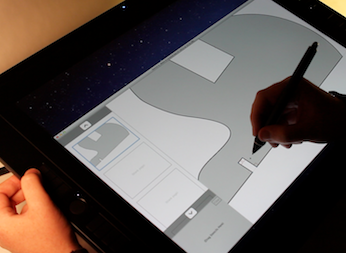
\includegraphics[width=0.6\linewidth]{img/simi-with-cintiq.png} % 0.65
}
\\
\subfloat[] {
   \label{fig:lg-pencil-holder}
   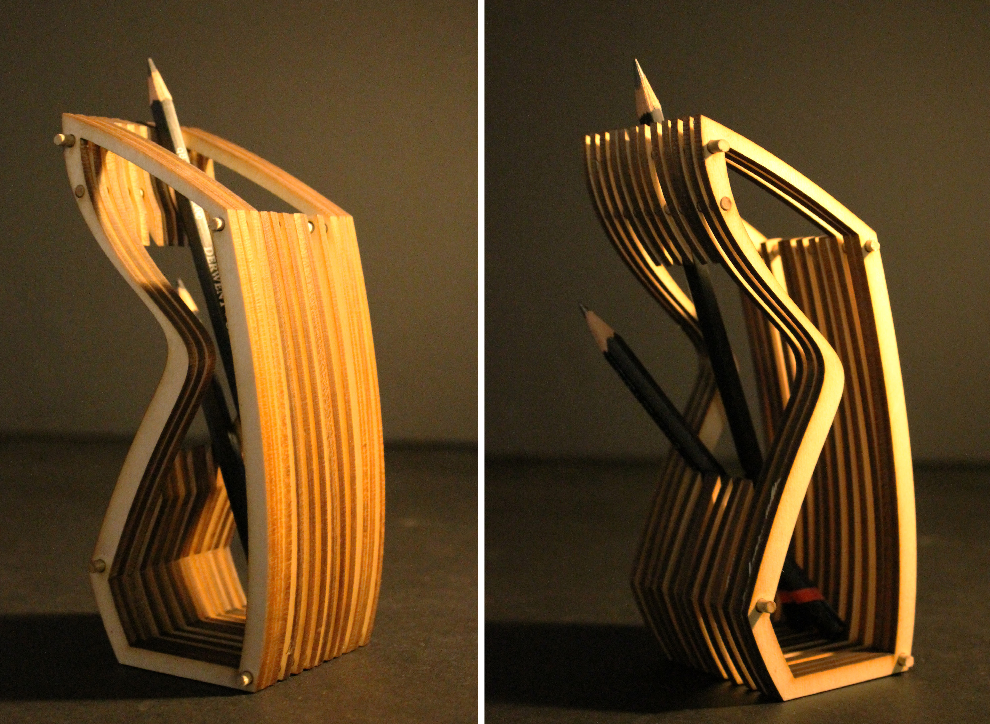
\includegraphics[width=0.6\linewidth]{img/lg-pencil-holder.png} % 0.9
}
\caption{Sketch It, Make It lets users design laser cut items with
  sketch-based interaction. \subref{fig:cintiq}: using SIMI with a
  Wacom Cintiq. \subref{fig:lg-pencil-holder}: laser-cut pencil
  holder designed by an undergraduate student using SIMI.}
\label{fig:simi-intro}
\end{figure}

A growing community of self-described \textit{Makers} design and build
many kinds of physical things~\cite{atlantic-rapid-fab}. Some are
electronic devices, while others are made entirely from traditional
materials. These ``new makers'' use rapid fabrication machines like 3D
printers, laser cutters, and other CNC machinery.

Laser cutters are among the more common and affordable fabrication
machines. One can think of a laser cutter as a fast, strong, and
precise automated razor that cuts flat material (paper, wood, plastic,
textiles, etc.). Many things can be made with only a laser cutter,
some fastened with screws or glue. Figures~\ref{fig:simi-intro}
and~\ref{fig:simi-example} show examples of laser cut objects.

Designers need modeling tools appropriate to their skills and
experience ~\cite{lipson-homefactory}. Today, designers can choose
from among several modeling tools for laser cutter projects. The most
common is Adobe Illustrator, a general-purpose, full-featured vector
graphics editor. Illustrator experts may find it a powerful and
convenient laser cutter design tool, but we observed that intermediate
users had substantial trouble using it when designing for laser
cutters.

Research on sketch-based modeling tools~\cite{johnson-sketch-review}
typically views sketching as an activity done mostly in the early
phases of design. Tools based on this assumption are justifiably
oriented towards capturing imprecise input; only a few sketch-based
systems support designers in later
stages~\cite{mori-plushie,saul-sketch-chair,naya-parsketch}.

We are inspired by the potential of freehand drawing as a basis for
precision modeling for several reasons. Sketching is quick and can be
easily learned. It is simple and modeless: unlike structured editing
software, a designer need not set a pencil's mode to line, circle, or
anything else. Yet (as we will show), sketched input can provide
enough information to make a precise digital model.

To support novice and intermediate designers, we present ``Sketch It,
Make It'' (SIMI), a modeling environment for laser cutter design based
on recognizing short sequences of input sketched with a stylus. Using
only freehand drawn input, SIMI enables a designer to iteratively and
incrementally create precise laser cut models.

\subsection{Motivating Example}

\begin{figure}[t]
\centering 
\subfloat[] {
  \label{fig:example-1} 
  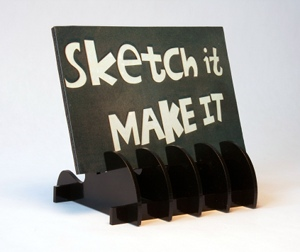
\includegraphics[width=0.45\linewidth]{img/simi-stand-withpic.jpg} 
}
\subfloat[] {
    \label{fig:example-2}
    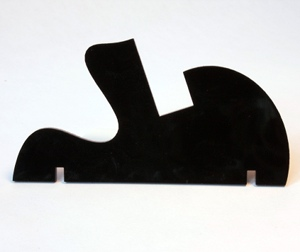
\includegraphics[width=0.45\linewidth]{img/simi-stand-part.jpg}
}
\caption{A picture stand \subref{fig:example-1} drawn and fabricated
  using SIMI. A single copy of the primary part is shown in
  \subref{fig:example-2}. }
\label{fig:simi-example}
\end{figure}

To introduce Sketch It, Make It we show how we use it to make the
picture stand shown in Figure~\ref{fig:simi-example}. We begin with
the idea of a stand with two horizontal rails as a base and a
five-part vertical support structure, joined with notches.

We first draw the rough profile of the vertical support piece using
curved and straight segments. SIMI captures our drawing, straightening
lines, smoothing curves, and connecting curved and straight segments.
 
After sketching the rough outlines of our two parts, we begin to
refine the design and make it precise.  We square the corners by
drawing right-angle braces (Figure~\ref{fig:motivating}a).  Now as we
adjust the shapes of the two parts by selecting and dragging endpoints
and re-shaping curves, SIMI maintains the right-angle constraints
we've established.
 
Next, we add notches to the two parts for the joints.  We draw five
small notches on the base rail.  For each notch we draw three lines
inside the outline of the part, and then use the erase gesture to
remove the residual outline segment (Figure~\ref{fig:motivating}b).
Then we indicate that both sides of the notch are to be the same
length: We draw tick marks on each segment, and right-angle braces to
keep the notch perpendicular to the edge of the part.  The notches
must have exactly the right dimensions: too wide, the top parts will
wobble; too narrow and they will not fit.  We size the notch by
overtracing its segments and entering fixed dimensions
(Figure~\ref{fig:motivating}c).
 
We drag the base part (twice) and the support part (five times) to
SIMI’s cut file area to prepare a PDF file for cutting, and then send
it to the laser cutter.  Finally we assemble the cut parts to make the
picture stand in Figure~\ref{fig:simi-example}.


\begin{figure}[t]
  \centering
  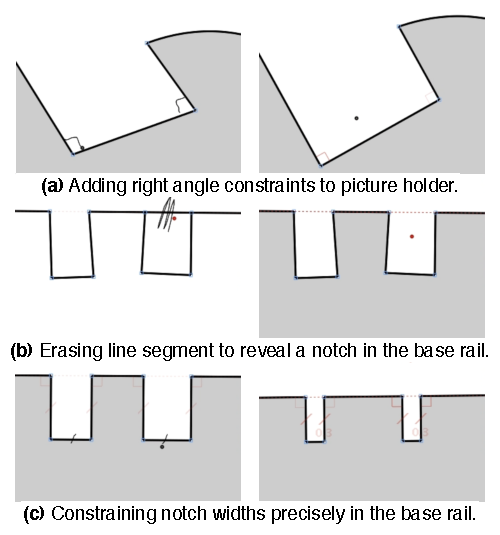
\includegraphics{img/motivating-example.pdf}
  \caption{Key steps taken when making the picture stand.}
  \label{fig:motivating}
\end{figure}

\subsection{Laser Cutting}

Laser cut designs are composed of parts cut from solid, flat material
and assembled in various ways: laminated, notched, bolted together,
\textit{etc}. Various materials require different laser speed and
intensity settings to achieve a quality cut. The designe uses a
software application to specify part shapes for laser cutting. The
software outputs vector graphics called a ``cut file'' that defines
these shapes. As most joints have small margins of error, lengths,
angles, and relative position must be specified precisely so that
parts fit together properly.

Tools for designing laser cut objects must allow users to precisely
specify dimensions. Like a physical saw, the laser leaves a gap in its
wake, called a \textit{kerf}, (between 0.2mm and 0.5mm on a 40 watt
cutter). This is an important consideration when designing facets
whose tolerances are small with respect to kerf. A notch joint, for
example, is ineffective if it is 0.1 mm too large or small.
\subsection{Organization}

We begin with a brief explanation of laser cutting followed by a
review of related work. We interviewed avocational designers about
using modeling tools and asked them to demonstrate how they use a tool
of their choice. We also analyze artifacts from two popular Maker
community web sites to identify features common among laser cutter
projects.

Second, we introduce \textit{Sketch It, Make It} (SIMI), a tool that
supports incremental sketch-based modeling for making precise 2D
shapes for laser cutting. SIMI provides a suite of mutually harmonious
pen interaction techniques to support the design process from a rough
sketch to precise, machinable output. Precision is achieved by
\textit{constraints} that maintain geometric properties such as
segment lengths and angles. We improve on existing sketch-based
interaction techniques (e.g., corner finding, recognition algorithms,
mode-switching), and bring them together in a fluid ensemble.

Third, we present an evaluation of SIMI in two parts---one with 60
first-year architecture students, the other, a task analysis comparing
SIMI with Illustrator. 

\section{RELATED WORK}

Two properties are common to many types of modern design work,
including design for laser cutters. First, designers sketch throughout
the process, especially (though not only) at the outset. Second, a
computer tool is used to render the design precisely. These properties
are common to diverse disciplines like graphic
design~\cite{wong-rr-prototypes}, automotive
engineering~\cite{kara-styling}, and software
development~\cite{mangano-software-whiteboard}. Sketching
is a powerful means for thinking and recording design intent, but as
many have observed, it is disconnected from the computer aided phase
of design and
manufacture~\cite{company-sketching-in-engineering}. SIMI helps close
that gap.

Sketchpad~\cite{sutherland-sketchpad} was a pioneering system that,
like SIMI, featured pen input and constraints for modeling shapes. The
user controlled Sketchpad's mode by pressing buttons with the
non-dominant hand, and drew on a display that sensed stylus
input. Because program mode was explictly established, the system
could readily process input directly without advanced recognition.

\subsection{Sketch-Based Design Tools}

The rough appearance of freehand sketches encourages designers to see
beyond unimportant details and make big-picture decisions. Much prior
work argues that beautification (e.g. redrawing crudely drawn lines as
straight segments) is antagonistic to design~\cite{gross-cocktail}, at
least during conceptual phases.

SILK~\cite{landay-silk-chi} is a sketch-based tool for prototyping
user interfaces. Sketching helps users avoid wasting effort on details
that are not yet important. For example, SILK lets designers place an
interface element without specifying its exact position and
size. Later, when the design is implemented, its position and size
must be given explicitly. However, as SILK is not designed for
precision, another system (e.g. a text editor) added to the tool chain
must be used. Once the designer's work shifts to later tools it is
inconvenient to revert to earlier tools. To eliminate this
discontinuity, we designed SIMI to support both ``sketching'' and
``making'' and to help the user fluidly transition from rough to
precise representations.

Some work takes the opposing view on beautifying sketched
input. Systems such as Pegasus~\cite{igarashi-pegasus} and recent work
by Murugappan \textit{et. al}~\cite{murugappan-beautification} enable
users to quickly and easily sketch simple vector drawings. These
systems infer the user's intention by detecting geometric
relationships. If more than one relationship is detected, the user
chooses among alternatives.

Inferencing is powerful, but it also prevents users from drawing
subtle distinctions. For example, an overly zealous inferencing engine
snaps objects together when the designer would like to place them near
one another. Therefore in SIMI, we keep automatic inference to a
minimum, and provide fast easy methods for correction.

Although users find sketch input an appealing way to interact with
computers, recognizers are not yet sophisticated enough to reliably
interpret arbitrary drawings. Therefore researchers have sought ways
to close the gap between input that people provide and the computer's
ability to make sense of it. For example a system may require users to
draw in certain ways (e.g. shapes must be drawn with single strokes,
as in SILK) to conform to the recognizer's capabilities.

Well known systems EverybodyLovesSketch and Teddy~\cite{bae-everybody,
  igarashi-teddy} introduced sketch-based interaction techniques that
are both easier for humans to use and for the computer to
process. They provide a small grammar of easy-to-make gestures to
create and edit 3D drawings. These systems are simple and powerful:
even children can learn and use them to make complex
models. EverybodyLovesSketch enables inexperienced users to create 3D
perspective concept sketches using a set of gestures and tools that
work well together.

However, it is hard to engineer with these tools because they do not
allow users to give precise and specific values for lengths and
angles. To address this shortcoming SIMI lets users set specific
values to sketched geometry.

\subsection{Sketch-Based Modeling for Fabrication}

Computer support for fabrication design has been a topic of interest
for decades, under the rubric of computer aided design (CAD) and
computer aided manufacturing (CAM). Most interaction is performed with
a keyboard and mouse, but this was not always so. For example,
SketchPad~\cite{sutherland-sketchpad} users controlled the design by
setting modes and parameters using one hand, while drawing on the
screen with a light pen in the other.

More recent interfaces enable users to model items for fabrication by
sketching. For example, Plushie~\cite{mori-plushie} users design soft
objects such as stuffed animals. They begin by creating 3D models of
bulbous objects by sketching shape outlines. The program outputs a
file of 2D shapes that users can cut from fabric, sew together, and
stuff.

Sketch Chair makes design for rapid fabrication more
accessible~\cite{saul-sketch-chair}. Users sketch the contours of a
chair's seat and back rest, and add legs. The system's physics
simulator lets the designer explore consequences such as if the chair
is stable.

Highly specific domain-oriented tools such as Plushie and Sketch Chair
are powerful because they enable inexpert designers to make things. A
few strokes are enough to define basic geometry, permitting Sketch
Chair to generate a seat. But those domain-oriented tools also make
important decisions like how the parts join. In contrast, SIMI users
specify as much or as little geometry as they want. But unlike Sketch
Chair and Plushie, SIMI has no built-in domain knowledge. It supports
a more general range of laser cutting, rather than a single class of
objects such as chairs or plush toys.

SIMI builds on the work of a small but interesting set of sketch-based
systems that support precision.  ParSketch~\cite{naya-parsketch} lets
users create parametric 2D models by incrementally recognizing
sketched geometry and commands. It uses pen pressure to distinguish
between linework (high pressure) and constraint commands (lower
pressure). Lineogrammer~\cite{zeleznik-lineogrammer} is a sketch-based
2D tool for drawing rectified vector graphics. Like
Pegasus~\cite{igarashi-pegasus}, it works on the principle of
interactive beautification, supporting iterative sketch/rectify
sequences. The interactive nature of these precision-oriented systems
allow the system to do less work when its recognizer/rectifier is
invoked, leading to higher accuracy.

Our work builds on this by providing (1) a collection of sketch-based
editing techniques that work well for incrementally specifying precise
details to an initially rough representation, and (2) the ability to
transition from a sketch into physical laser-cut output.

\section{FORMATIVE STUDIES}

To better understand the tasks and problems designers face when
designing for laser cutters, we conducted two related formative
studies.  In the first, we interviewed people with experience
designing these artifacts and watched them work. In the second, we
surveyed and analyzed laser-cut items found on community web sites to
identify common features.

\subsection{Formative Study on Designer Work Practices}
\label{sec:formative}

We interviewed six designers from different backgrounds, including
mechanical engineering, graphic design, and architecture to learn
about their work practices and to understand how they use their
tools. All were experienced with designing objects to be made with a
laser cutter.

Each session lasted approximately one hour, split evenly between an
interview and using software. We met participants in their workplaces,
and asked them to describe their design process and to show sketches
or videos of their work. Although there were differences in their
process, each followed the same overall pattern.

The designers all said they began by thinking about a problem and
sketching on paper. They made drawings to think about how to ``frame''
the project (what it is for). Other sketches helped reason about how
to make it (how it works and fits together). Some designers explicitly
noted that sketching is a necessary part of the process: they could
not move forward without making freehand drawings. Only after the idea
is well-formed were they ready to translate their hand-made sketch
into a computer model (Figure~\ref{fig:translate}).

\begin{figure}[h]
  \centering
  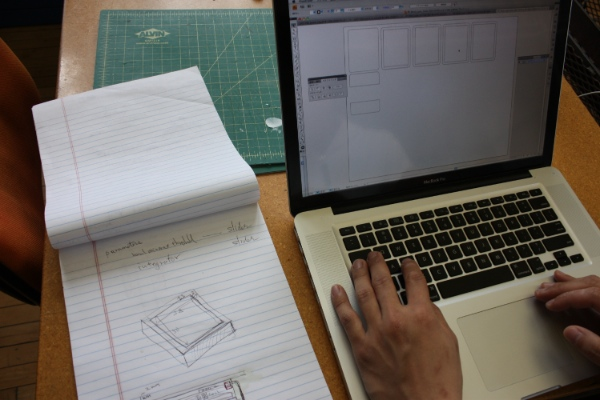
\includegraphics[width=0.7\linewidth]{img/translate-sketch-to-computer.jpg}
  \caption{A common step of designing for laser cutters: translating a
    hand-made sketch to a computer modeling tool. The sketch includes
    a perspective drawing of the desired result, and 2D diagrams of
    individual parts with key dimensions indicated.}
  \label{fig:translate}
\end{figure}

After the interview, we asked participants to copy the sketch shown in
Figure~\ref{fig:interview-sketch} using a software tool of their
choice. We wanted to learn what problems people encountered when
executing the common task of translating a sketch to a computer model.

\begin{figure}[h]
\centering \subfloat[We asked users to replicate this sketched part.]
           {
  \label{fig:interview-sketch-1} 
  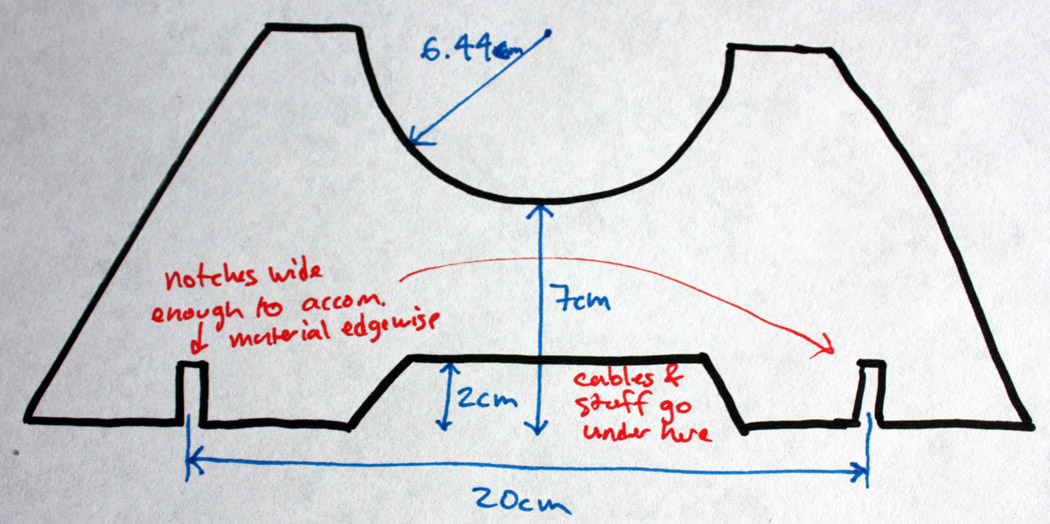
\includegraphics[width=0.7\linewidth]{img/laser-me-1.jpg}
}

\subfloat[Drawing of the part in context.] {
    \label{fig:interview-sketch-2}
    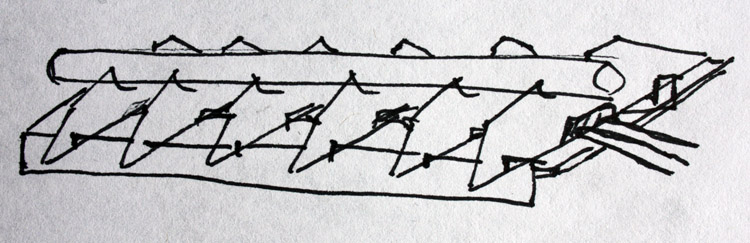
\includegraphics[width=0.7\linewidth]{img/laser-me-2.jpg}
}
\caption{We asked participants to model the part at the top using
  a software of their choice.}
\label{fig:interview-sketch}
\end{figure}

Five participants chose to implement the sketch with Illustrator; one
chose Rhino. All users were comfortable with their tools, but none
were experts. Every designer's strategy involved common activities:
creating and editing boundaries, aligning or snapping items, using
guide lines or reference points, measuring distances, specifying or
changing lengths and angles, and creating finished ``cut files'' to
send to the laser cutter.  They also engaged in the usual interaction
management tasks---selecting and deselecting on-screen elements, and
view port management such as zooming and panning.

Participants spent a good deal of time on operating overhead
(approximately 50\%). This included searching for the appropriate tool
for the next task and recovering from errors. For example, one
designer, an experienced Illustrator user, was aware of the ``Path
Finder'' tool and wanted to use it. He searched the program's menu
structure and hovered over toolbar buttons to read tool tips. Next, he
invoked various functions of the Path Finder, using the keyboard
shortcut to undo after each failed attempt, as he searched for the
correct mode within the subcommand palette. This process lasted
approximately 80 seconds.

Occasionally participants used features in unorthodox ways. For
example, to remove an unwanted segment of a polyline, one participant
(a graphic designer) created an opaque white rectangle to obscure it,
rather than erase it. (``Don't tell anyone I did this'', he said).

Similar episodes are common: a person \textit{should} know the
`correct' action, but takes an alternate approach. Although the
alternative achieves the intended effect, it might be less efficient
(more operations, longer execution time) or introduce unwanted
complexity (e.g. the white rectangle).

In short, we found that most common tasks and problems belong to three
main groups:

\begin{itemize}
\item \textit{Defining geometry:} Creating/editing boundaries,
  aligning items, creating and using guide lines or reference points,
  measuring distances, and specifying lengths or angles.
\item \textit{Managing the editing tool:} Selecting/deselecting
  objects, view port management, finding and entering tool modes, and
  recovering from errors.
\item \textit{Cut file:} Finalizing the cut file by creating copies of
  items when more than one is needed, and positioning stencils.
\end{itemize}

\subsection{Artifact Feature Analysis}

The formative study of work practices from the previous section helps
us understand \textit{how} people create laser cut items. To learn
more about the characteristics of those objects (\textit{what} people
create), we analyzed finished items from two web-based communities of
laser cutter users.

Many users are motivated by the opportunity to share their designs
with others. Ponoko and Thingiverse are two currently popular web
sites for selling or sharing items that can be made with rapid
fabrication machines. Ponoko offers thousands of user-designed items
for sale, mostly produced by laser cutting. Thingiverse is a warehouse
of digital models of 3D-printable objects and designs for laser
cutters. From these two sites we selected a total of 55 laser-cut
designs. On Ponoko we selected the most recent 45 laser cut items.  On
Thingiverse we searched for objects with the ``laser cutter'' tag and
selected ten. Figure~\ref{fig:ponoko} summarizes the feature analysis
of these 55 projects.

\begin{figure}[h]
  \centering
  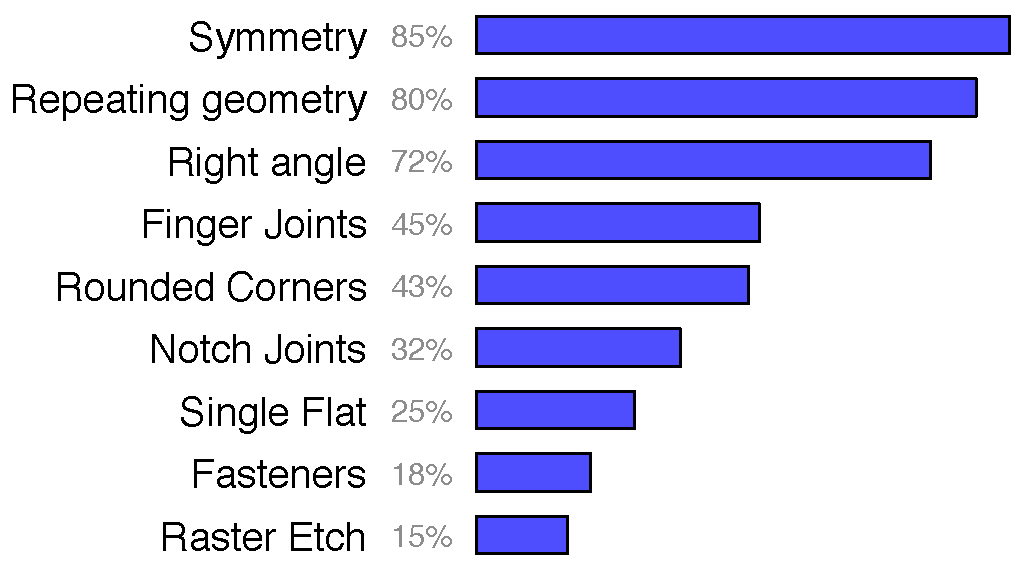
\includegraphics[width=0.9\linewidth]{img/ponoko-graph.pdf}
  \caption{Frequency of features of 55 laser-cut designs found on
    Ponoko and Thingiverse.}
  \label{fig:ponoko}
\end{figure}

We used ten properties to characterize each project, based on our own
experience designing objects for laser cutters, as well as
observations from the formative study. They are:

\begin{itemize}
\item \textit{Symmetry}: Radial/linear symmetry is present.
\item \textit{Repeating geometry}: Linework is repeated several times.
\item \textit{Right Angle}: Edges meet at 90-degree angles.
\item \textit{Notch and Finger Joints}: Two parts come together using one of
  the joints illustrated in Figure~\ref{fig:joint}.
\item \textit{Rounded Corners}: Right-angle corners are slightly blunt.
\item \textit{Splines}: Curved linework (not counting rounded corners).
\item \textit{Single Flat}: The project is composed of a single, flat
  piece of material (e.g. a coaster).
\item \textit{Fasteners}: Use of glue, screws, or bolts.
\item \textit{Raster etch}: Laser cutter etched patterns (e.g. words,
  images) rather than cutting all the way through material.
\end{itemize}

This list of properties helped us decide what SIMI should (and should
not) do. Our implementation is discussed next.

\begin{figure}[h]
\centering 
\subfloat[Notch joints.] {
  \label{fig:joint-notch} 
  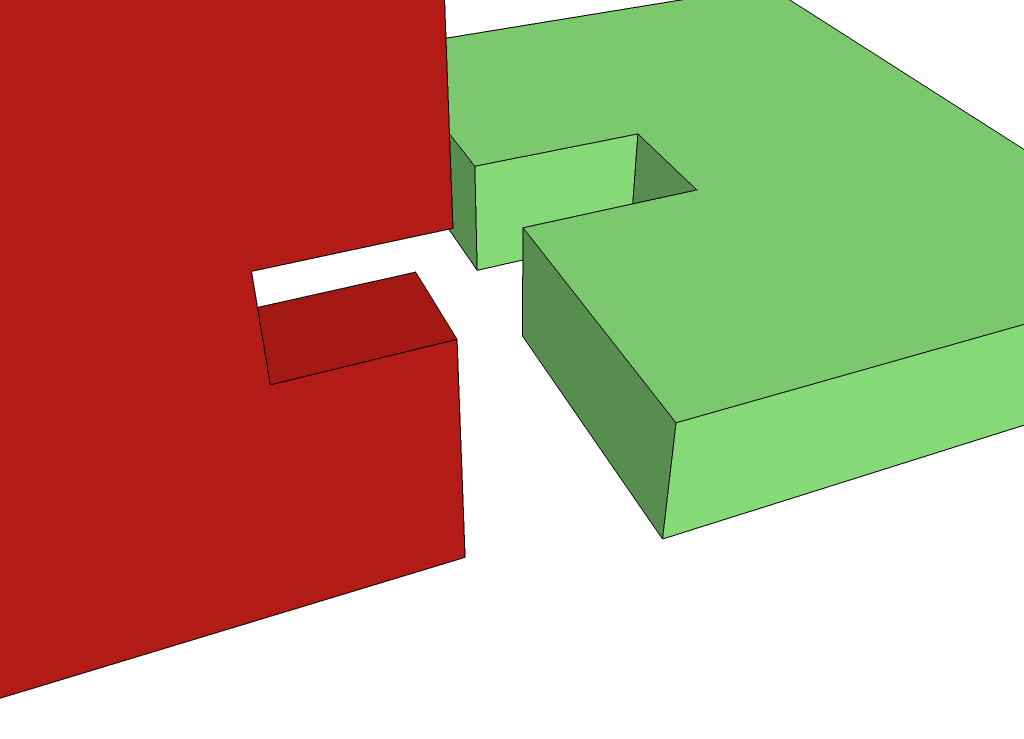
\includegraphics[width=0.4\linewidth]{img/joint-notch.png}
}
\subfloat[Finger (box) joints.] {
    \label{fig:joint-finger}
    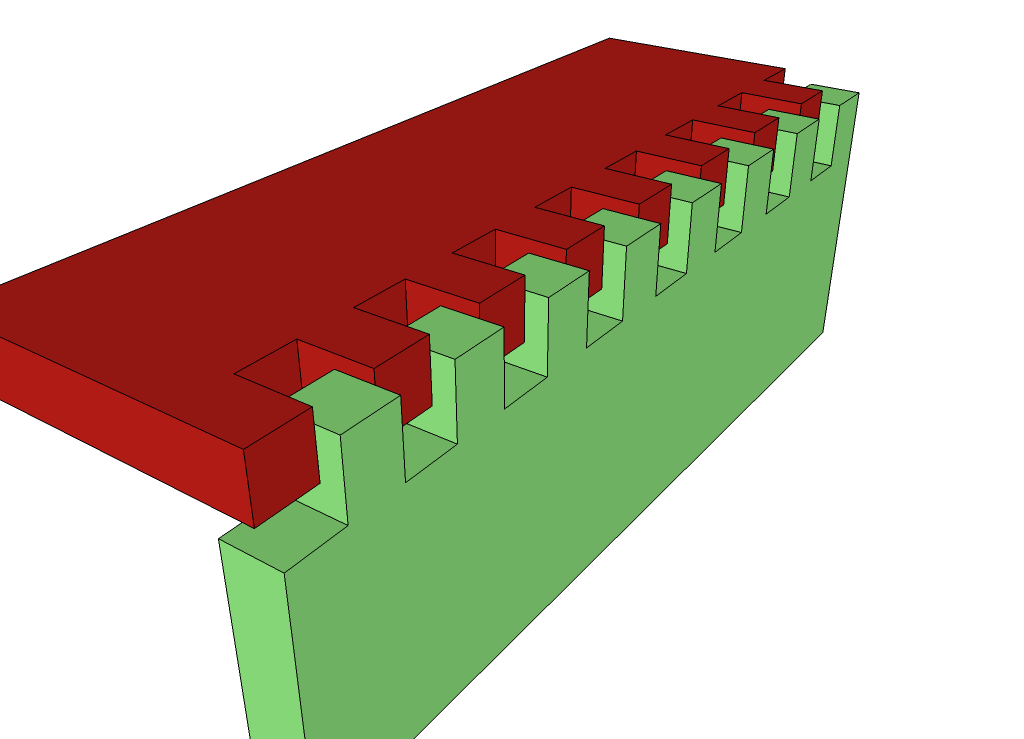
\includegraphics[width=0.4\linewidth]{img/joint-finger.png}
}
\caption{Two common methods to join parts. Notch joints are used when
  parts intersect along part midsections; finger joints (box joints)
  join parts along edges.}
\label{fig:joint}
\end{figure}

\section{SKETCH IT, MAKE IT}

Based on the designer's work practices (formative study) and the
artifacts they make (feature analysis), we developed \textit{Sketch
  It, Make It} (SIMI), a 2D sketch-based tool for modeling laser cut
items. We aim to address problems with current modeling systems and
support the most common practices with a tool to specifically support
designing laser-cut items. However, we also believe that the
techniques illustrated here have broader applicability beyond laser
cutting. 

Design for laser cutting requires precision. SIMI addresses this with
user-created constraints---geometric relationships between two or more
items. For example, two lines can be constrained to meet at a common
point, and then constrained to meet at a right angle. Constraints are
maintained as the user edits a model. With same-length, same-angle,
and right-angle constraints users create objects with symmetric or
repeating geometry. (Details on constraints and our custom-built
constraint engine are provided below.)

We can think of design with SIMI as three phases: \textit{Create},
\textit{Constrain}, and \textit{Cut}. In the Create phase, the
designer draws freehand strokes. In the Constrain phase, the user adds
precision by specifying geometric relationships and dimensions. And in
the Cut phase, the designer builds a cut file for fabrication. As SIMI
supports all three phases, the designer can move back and forth at any
time.

Users draw with a stylus, and use a button with their other hand for a
few actions. The system recognizes input as either geometric linework
or gestural commands. Linework includes straight lines, elliptical
arcs, splines (open-ended or closed shapes), circles, and
ellipses. There is no tool palette---users invoke commands to operate
on linework by drawing gestures. Some gestures are recognized and
execute immediately, such as the erase (scribble) gesture. Other
gestures (such as those that establish constraints) are recognized
after the user presses the button, or after a timeout.

Perhaps the greatest distinction between SIMI and prior sketch-based
design tools is that users can accurately specify geometry. This is
done by setting distances and angles to specific values. However to
allow for early design in which precision can actually be a
disadvantage, the user need not specify details until they become
important. The systems does not \textit{require} users to attend to
detail, but enables a designer to transition smoothly from a rough
imprecise model to a specific precise model via sketch interaction.

SIMI recognizes a closed 2D path as a `stencil'. Stencils are shapes
that can be placed on the virtual laser cutter bed. Several copies of
a stencil can be added. The system generates a vector file for laser
cutting. 

\subsection{Sketch Interaction Techniques}

Guiding the development of SIMI is the principle that the designer
need never set down the pen. Input is provided entirely with a stylus
except for a single button used by the non-dominant hand to access
additional commands. The gestures used to invoke commands or add
constraints are summarized in Table~\ref{tab:gestures} and described
in detail in the following sections.

\begin{table}[h]
\centering
\begin{tabular}{ p{2.25cm} p{5.5cm} }
\textbf{Gesture} & \textbf{Remark} \\
\hline
Latching & Make segments share a common point.\\
Erase & Remove unwanted segments.\\
Same Length & Constrain line lengths to be equal.\\
Specific Length & Constrain line lengths to a value. \\
Right Angle & Constrain two lines to a $90\,^{\circ}$ angle.\\
Same Angle & Constrain two angles to be equal. \\
Flow Selection & Deform and smooth curved segments.\\
Undo and Redo & Browse and revert design history.\\
Camera Control & Zoom and pan.\\
\end{tabular}
\caption{Summary of SIMI's gestures.}
\label{tab:gestures}
\end{table}


\begin{figure}[h]
\centering \subfloat[Automatic: latch when endcaps intersect
  (shaded extensions).] {
  \label{fig:latch-auto} 
  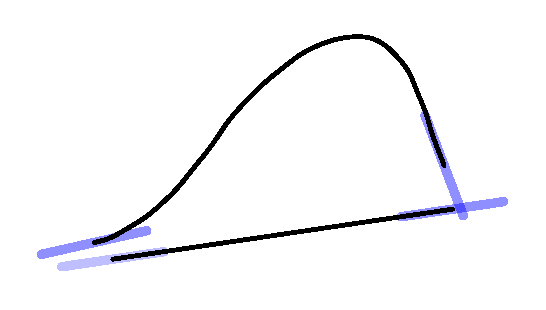
\includegraphics[width=0.43\linewidth]{img/latch-auto-endcaps.pdf}
}\hspace{3mm}
\subfloat[Endpoint latching.] {
  \label{fig:latch-endpoint} 
  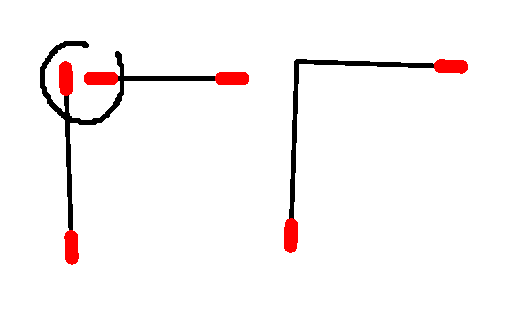
\includegraphics[width=0.43\linewidth]{img/latch-manual-endpoint.pdf}
}
\\
\subfloat[Continuation latching.] {
    \label{fig:latch-continuation}
    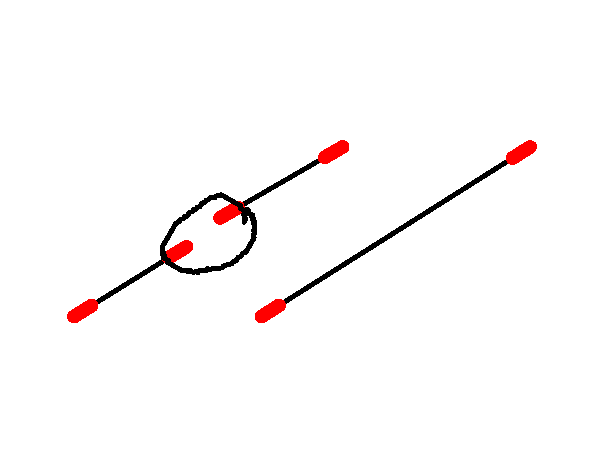
\includegraphics[width=0.43\linewidth]{img/latch-manual-continuation.pdf}
}\hspace{3mm}
\subfloat[T-Junction latching.] {
    \label{fig:latch-tjunct}
    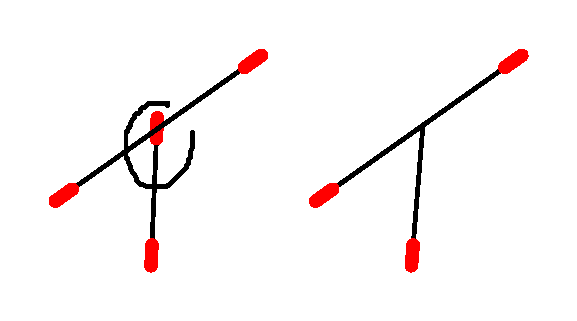
\includegraphics[width=0.43\linewidth]{img/latch-manual-tjunct.pdf}
}
\caption{Automatic and manual latching brings segments together to
  meet at a common point.}
\label{fig:latch}
\end{figure}

\subsubsection{Latching}

Users often want lines to meet at a common point. In the formative
work practices study, we observed Illustrator users struggling to make
lines co-terminate. Sometimes the designer would simply extend lines
past each other to ensure that the laser will correctly cut the
corner.

Latching is the process of adjusting adjacent segments (lines,
splines, arcs, \textit{etc.}) to meet at a common
point~\cite{herot-latch-corners}. SIMI provides two methods for
latching segments, illustrated in Figure~\ref{fig:latch}. One is
automatic: the system analyzes new linework for cases where the user
likely meant their segments to connect, and adjusts one or more
segments to meet. Automatic latching can pose problems if it is too
zealous. Therefore our latcher is intentionally conservative to avoid
frustrating users. SIMI's second latching method is manual: the user
draws a small circle around the endpoints to be latched.

All linework in SIMI is meant to compose stencils, which are closed
sequences of latched segments. The designer must be able to find and
fix un-latched segments to make stencils. To reveal un-latched
segments, SIMI draws a red marker at lonely endpoints.

Three different spatial arrangements can be latched: endpoint latching
(corners), continuation, and T-junctions (see
Figure~\ref{fig:latch}). Endpoint
latching~(Figure~\ref{fig:latch-endpoint}) is what the automatic
latcher does. Continuation
latching~(Figure~\ref{fig:latch-continuation}) brings together two
segments that have nearly the same direction at the joined point,
replacing two segments with a single larger segment. A
T-junction~(Figure~\ref{fig:latch-tjunct}) latches one segment
endpoint to the middle of another, splitting the second segment in
two.

\subsubsection{Erase}

\begin{figure}[h]
  \centering
  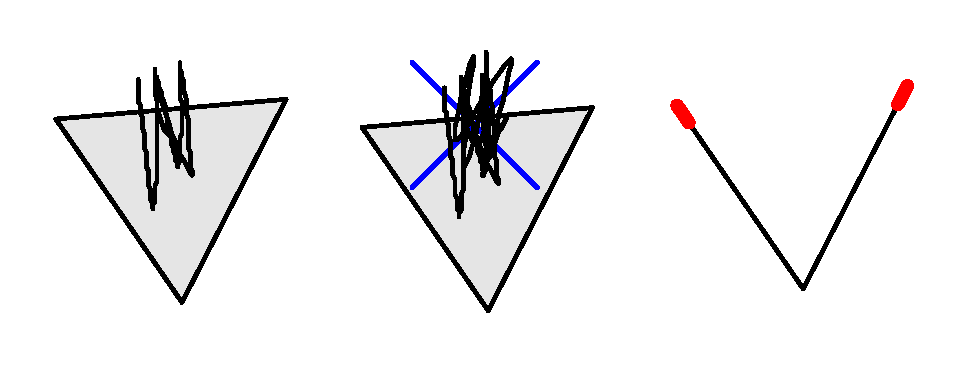
\includegraphics[width=0.9\linewidth]{img/erase-all.pdf}
  \caption{Erase gesture: before, during, and after.}
  \label{fig:erase}
\end{figure}

Users may want to remove linework for various reasons: to delete
unwanted or accidentally drawn lines, or as part of a deliberate
strategy to cut away geometry allowing new shapes to
emerge~\cite{zeleznik-lineogrammer}. Like latching, erasing is a
common task so it is invoked with a simple scribble gesture made over
the linework to be erased.

Our algorithm for detecting erasure executes efficiently during the
pen stroke. As soon as SIMI detects that the user is making an erasure
gesture, it provides visual feedback mid-stroke to signal users their
erasure will succeed. Figure~\ref{fig:erase} shows an erase gesture
with the visual feedback.

\subsubsection{Angle and Length Constraints}

Most laser cut items employ right angles, symmetry, and repeated
geometry (see Figure~\ref{fig:ponoko}). Designers can create stencils
with these properties by imposing constraints.

\begin{figure}[h]
  \centering
  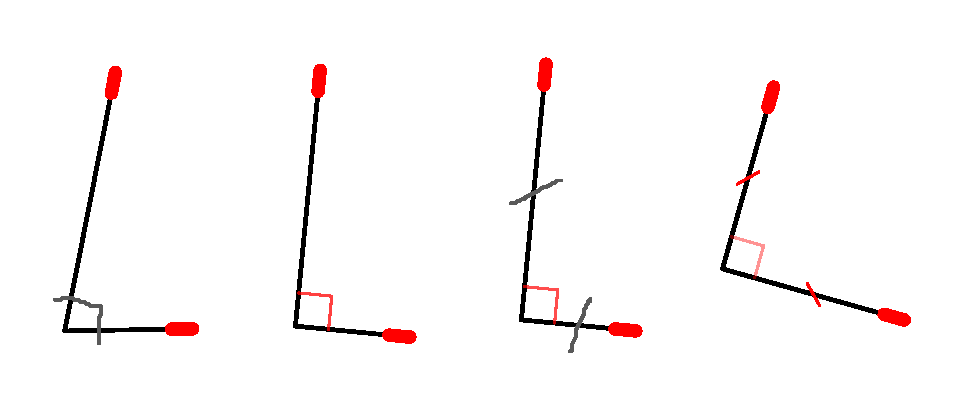
\includegraphics[width=0.9\linewidth]{img/constraints-all.pdf}
  \caption{Gestures for adding a right angle (left) and same-length.}
  \label{fig:constraints}
\end{figure}

In SIMI, designers add constraints by marking up the
linework. Traditional drafting and standard geometry diagrams indicate
a right angle with a brace symbol at the intersection of the two
edges. SIMI recognizes drawn input that looks like that brace and adds
a constraint on the associated segments
(Figure~\ref{fig:constraints}).

Another drafting convention uses tick marks (hash marks) to indicate
that lines have the same length. SIMI recognizes tick marks crossing line
segments as a gesture to create a \textit{same-length constraint}.

SIMI also lets designers set specific lengths, invoked by selecting a
line (by over-tracing a portion of it) and typing a number (for now we
allow keyboard input for this one case; handwriting support is future
work). 

Angles can be constrained to be equal with the same tick mark gesture
used to make lines the same length.

\subsubsection{Flow Selection}

% Justify wrt user study and Ponoko analysis

About one-third of the models examined in our laser cut artifact
analysis involved curves (splines). SIMI provides Flow
Selection~\cite{johnson-flow-selection} to enable users to create and
modify splines (Figure~\ref{fig:fs}). The user `heats up' portions of
curved segments by holding the pen down near the curve. Then, without
picking up the pen, the user deforms the heated region by
dragging. ``Hotter'' points move more.

\begin{figure}[h]
\centering \subfloat[Selecting (``heating'') points along a curve. The
  selection grows while as the stylus is down. ] {
  \label{fig:fs-1} 
  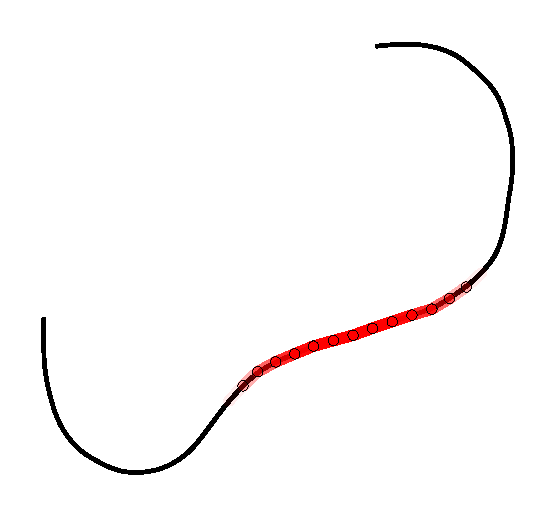
\includegraphics[width=0.4\linewidth]{img/fs-1.pdf} }
\hspace{3mm} \subfloat[Deforming the region by moving the
  stylus. ``Hotter'' points (close to the pen) are moved more.] {
  \label{fig:fs-2} 
  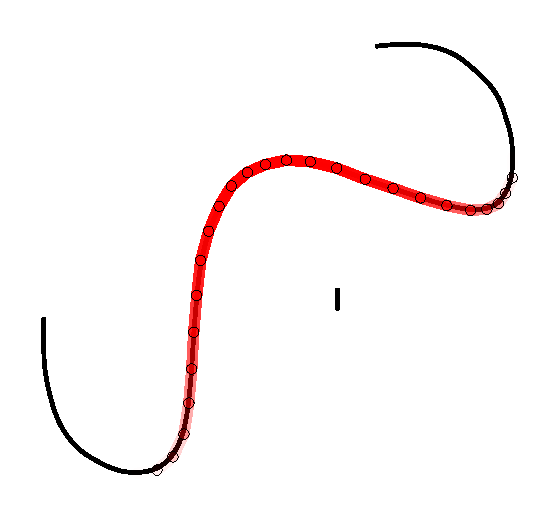
\includegraphics[width=0.4\linewidth]{img/fs-2.pdf}
}
\caption{Flow selection is used to deform curved segments. By holding
  the pen down, SIMI enters a transient mode that slowly heats the
  segment near the stylus. When the pen moves, the heated points move
  with it.}
\label{fig:fs}
\end{figure}

\subsubsection{Undo and Redo}

SIMI provides a novel means of performing Undo and Redo that lets
designers browse the entire history of the drawing using a single pen
stroke. Participants in the formative evaluation used the Undo and
Redo features of Illustrator and Rhino in two distinct ways: to revert
state following epistemic actions, or to recover from usability
problems~\cite{akers-undo}. First, Undo gives designers confidence to
modify their work to explore alternative designs. Epistemic
actions~\cite{kirsch-epistemic-action} are taken to ask ``what if''
questions, like rotating an object 90 degrees to see if it that
orientation is better. Such actions support creative exploration. If
the designer does not like their modifications they Undo to a prior
state. The second class of Undo events stems from errors: either
usability problems or user error.

Users undo by pressing the offhand button and dragging the pen
left. Every 40 pixels left triggers one undo action. Dragging farther
to the left undoes several times. Redo is done by dragging to the
right. Both undo and redo may be triggered by the same stroke by
changing direction, letting designers scan the drawing history for a
desired state. The vertical dimension is not used in the undo or redo
gesture.

\subsubsection{View Port Control}

SIMI lets users control the view port. Tapping the pen twice displays
a pan/zoom widget shown in Figure~\ref{fig:panzoom}. To pan, drag
starting in the left square in any direction. To zoom, start in the
right square: up to zoom in, down to zoom out (the horizontal
dimension is not used). The controls disappear after two seconds of
non-use.

\begin{figure}[h]
  \centering
  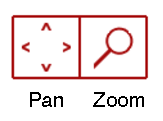
\includegraphics[]{img/panzoom.pdf}
  \caption{The pan/zoom widget is invoked by double-tapping the
    pen. Dragging in either square changes the viewport by panning
    (left square) or zooming (right square).}
  \label{fig:panzoom}
\end{figure}

\subsection{Constraint Engine}

SIMI users can establish \textit{constraints} that enforce geometric
relationships in a drawing. For example, the user might draw a
triangle and establish a right angle constraint. As the user
manipulates the triangle (moving vertices or changing segment
lengths), our constraint engine maintains that particular corner as a
right angle.

SIMI's custom-built constraint engine is an iterative, numeric solver
that minimizes the total error of all constraints. Each constraint's
error is computed as how far each related point must move. To manage
contending constraints, the system computes a change vector for each
point by computing the change required by all related
constraints. Each point moves a small amount along its change vector,
and the process continues until the total error becomes minuscule.

The solver can get trapped in a loop as points oscillate between
several values. We use simulated annealing~\cite{metropolis-annealing}
to avoid this case: we add entropy to move points randomly. Gradually
the system reduces entropy and the points settle to a satisfactory
configuration.

\subsection{Stencils}

SIMI's final product is a ``cut file'': a vector drawing for output on
a laser cutter. This cut file typically contains a number of
stencils---closed 2D shapes that define the laser's path. Stencils may
have complex boundary geometry with non-intersecting edges. Stencils
can also have holes in them for joints, fasteners, or other purposes.

To identify stencils, SIMI forms a graph with segments as edges and
their endpoints as nodes. It then runs a depth-first search. Each
cycle is a candidate stencil; the algorithm eliminates all subgraph
cycles, retaining the outer linework comprising the cutout. Stencils
are visually represented by shading their interior.

\section{SYSTEM EVALUATION}

We evaluated Sketch It, Make It in two ways. First, we tested SIMI
with 60 undergraduate architecture students. Our objective was to test
if (and how well) SIMI's sketch-based interaction could be used to
make precisely-defined designs for fabrication. Second, we compare an
experienced SIMI user's strategy for making an object with that of an
experienced Illustrator user. We did this to compare how these starkly
different tools require designers to work.

\begin{figure}[t]
\centering \subfloat[Questions about features: attitude and ease of
  use.] {
  \label{fig:survey-feature-ease-attitude} 
  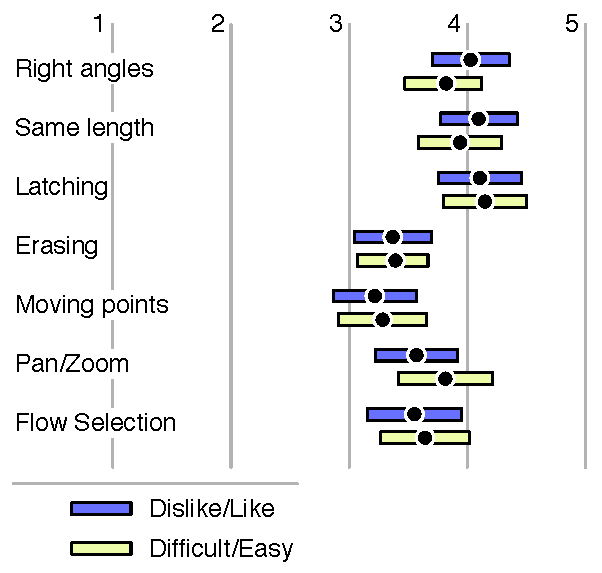
\includegraphics[width=0.9\linewidth]{img/feature-attitude-and-ease.pdf}
}
\\
\subfloat[Questions on the system as a whole.] {
    \label{fig:survey-program-attitude}
    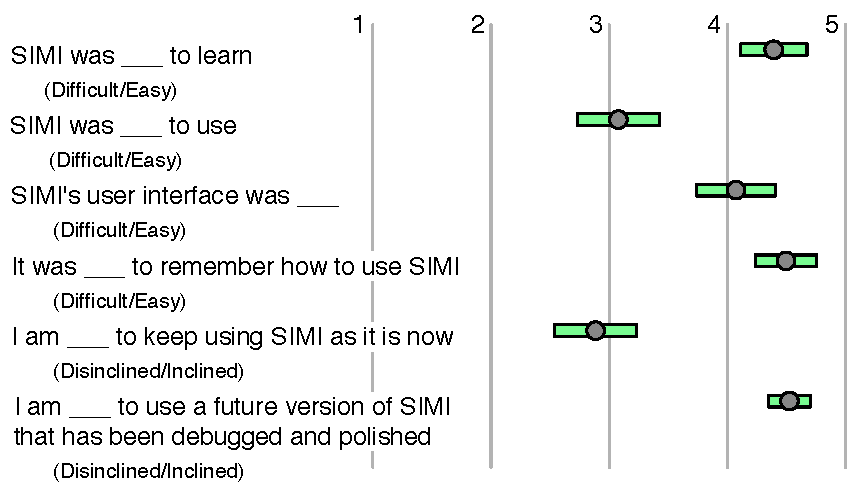
\includegraphics[width=0.9\linewidth]{img/program-attitude-2.pdf}
}
\caption{Survey results from the workshop with undergraduate
  architecture students. 40 students responded to the questionnaire.}

\label{fig:survey}
\end{figure}

\subsection{Student Workshop}

We held a workshop with 60 undergraduate architecture students to
gather qualitative feedback about how easy or difficult SIMI is to
learn and use. The primary author ran the workshop in 30-minute
sessions over two days in a room equipped with iMacs and Wacom Intuos
tablets. Regrettably, these tablets do not display output, so users'
eyes are not focused on the same physical location as the pen
tip---leading to significant hand-eye coordination challenges. More
costly display tablets like the Cintiq (Figure~\ref{fig:cintiq}) avoid
this problem, but were unavailable for our workshop.

Initially, students complained that the tablet hardware was difficult
to use, but they acclimated to it after about ten minutes. Then they
quickly learned to make linework and constraints. At first they had
trouble erasing and using control points, but soon learned to make
these gestures.

We expected students to have difficulty using SIMI because the
hardware (tablets) and interaction paradigm (sketch-based modeling)
were both new to them. However, by the second day, most questions and
comments regarded missing features, not about how to use the system.

After the workshop, students were offered an extra credit assignment
to complete a short survey. This generated 40 responses, summarized in
Figure~\ref{fig:survey}. The survey had three sets of questions, all
on a 5-point scale. The first set asked how easy (or hard) each
interaction method was to use. The second set of questions measured
the student's attitude about the techniques. This line of questioning
was borrowed from~\cite{bae-everybody}.

Only the Erase and Control Dot gestures seemed to give participants
trouble. These are the only gestures that depend on timing. Erasing
must be done with a quick, vigorous shake of the pen. Control dots
must be made quickly, or SIMI will interpret the input as the
beginning of a flow selection.

The last set of questions polled students about their perception of
the program as a whole: e.g. how easy it was to learn, to use, and
remember. Although the students reported the system was easy to
\textit{learn}, their responses indicate they found it difficult to
\textit{use}. This might be explained by the limited time available
(one hour), and the novelty of the hardware.

Finally, we asked (1) how much people would like to continue using the
system as it is currently, and (2) how likely they would be to try it
again when it was debugged and nicely tuned. The responses are in
stark contrast: most would not continue using SIMI as it is today,
owing to bugs and lack of features. Despite this, the response to the
second question was very positive.

Enthusiasm about the interaction paradigm of sketching was evident in
comments by respondents. For example:

\begin{itemize}
\item ``This is the start of a great program, and once it is polished it
  will be extremely useful.''
\item ``The program seems like it could be really cool to use in the
  future. I really enjoyed using a tablet and stylus. It made
  designing fun.''
\end{itemize}

Not all commentary was positive. Aside from complaints about bugs,
most negative comments concerned missing features (for example, a
constraint to make lines parallel).

\subsection{Task-Tool Analysis}

A second method to evaluate our system is to compare the actions
required to make an object with SIMI compared with those of a
conventional tool such as Illustrator.

We asked an expert Adobe Illustrator user to verbally describe the
sequence of discrete actions necessary to model the parts of the table
shown in Figure~\ref{fig:table}. This designer has used Illustrator to
make dozens of laser-cut items.

\begin{samepage}
For example, the first three actions were:

\begin{enumerate}
\item Press the M key to enter rectangle drawing mode.
\item Type rectangle dimensions.
\item Place the rectangle on the drawing canvas.
\end{enumerate}
\end{samepage}

The first action is a persistent mode change, while the second two
specify values. A similar transcript was recorded for SIMI (the
primary author provided the protocol).

We identified discrete actions from the verbal protocol, and coded
each using five categories:

\textit{Persistent mode change}: Change the tool input state so
subsequent input is interpreted in context of that tool (e.g. line
drawing mode). User must enter another persistent mode to exit the
first.

\textit{Specify value}: Specify a dimension or location.

\textit{Specify target}: Indicate (select) an element for a subsequent
operation.

\textit{Transformation}: Apply an operation that changes existing
model elements (e.g. move or erase something)

\textit{Transient mode change}: Temporarily change the tool mode so
input is interpreted differently. This kind of mode change is part of
a phrase, and will revert to another mode when the phrase is complete.

\begin{figure}[h]
  \centering
  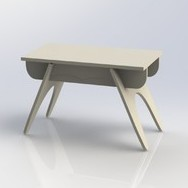
\includegraphics[width=0.4\linewidth]{img/table.jpg}
  \caption{A laser-cut table for sale on Ponoko. We asked expert
    designers how they would replicate this object using either
    Illustrator or SIMI.}
  \label{fig:table}
\end{figure}

\begin{table}[h]
\centering
\begin{tabular}{ l c c }
\textbf{Action type} & \textbf{Illustrator} & \textbf{SIMI} \\
\hline
Persistent mode change & 12 & 0 \\
Specify value & 17 & 7 \\
Specify target & 7 & 4 \\
Transformation & 6 & 27 \\
Transient mode change & 2 & 0 \\
\hline
& \textbf{44} & \textbf{38} \\
\end{tabular}
\caption{Frequency of action types in the design protocol of expert
  Adobe Illustrator and SIMI users. }
\label{tab:expert}
\end{table}



The action frequency (listed in Table~\ref{tab:expert}) shows how the
two tools are used to create the same output. Roughly the same number
of actions was taken (Illustrator:~44, SIMI:~38).

To make an object using Illustrator, an expert issues a series of
\textit{Select, Specify} actions: either activate a persistent tool
(e.g. line mode) or select a modeling element (e.g. a line on the
screen), then specify a value or position by typing a number or moving
the mouse.

In contrast, most discrete actions with SIMI involve transforming
geometry that is already on the screen, for example, constraining two
existing lines to meet at a common point or form a right angle. A
single sketched gesture fluidly performs both \textit{Select} and
\textit{Specify} operations that require two distinct actions in
Illustrator. For example, right angle gesture necessarily indicates
the line segments to be constrained.

\section{IMPLEMENTATION}

SIMI is programmed in Java. It uses the Java binding for OpenGL (JOGL)
for graphics and NIST's JAMA package for linear algebra. When packaged
as a self-contained executable, the Mac OS X application is 8.2
megabytes.

\section{FUTURE WORK}

We continue to improve SIMI. Beyond fixing bugs and improving
responsiveness, we will develop sketch-based techniques to add
functions requested during the workshop. These include parallel and
specific-angle constraints, and the ability to move, rotate, and scale
objects.

Currently users provide numeric input with the keyboard. We will add
handwriting recognition. To make SIMI models parametric, we will also
support variables and simple algebraic expressions in addition to
numbers.

We would like to make it easier to create long sequences of repeated
geometry (e.g. jagged pattern in Figure~\ref{fig:joint-finger}'s box
joints). One approach is to use shape replacement: let the user draw
or select simple geometry, and pick a replacement from a
library. Another approach is to let users define \textit{hints} for
pattern recognizers. For example, selecting the lines comprising a
notch would create a short-term hint to the sketch recognizer. Input
that looks like the hint would be rectified as the selected notch.

\section{ACKNOWLEDGMENTS}

% TODO: fill this in later. Leave left blank for blind review.

Acknowledgments...
\newpage

\bibliography{simi}

\end{document}
